\documentclass[a4paper,12pt]{report}
\usepackage[top=2cm, bottom=2cm, left=1cm, right=1cm]{geometry}\usepackage[T1]{fontenc}
\usepackage[utf8]{inputenc}
\usepackage{lmodern}
\usepackage{amsmath}
\usepackage{amsfonts}
\usepackage{amssymb}
\usepackage{amsthm}
\usepackage{graphicx}
\usepackage{color}
\usepackage{xcolor}
\usepackage{url}
\usepackage{textcomp}
\usepackage{parskip}
\usepackage{hyperref}
\usepackage{listings}
\usepackage{float}
\usepackage{tikz}
\usepackage{multicol}
\usetikzlibrary{automata, positioning, arrows}
    
\lstset{basicstyle=\ttfamily\footnotesize,breaklines=true}
    
\title{ECE 385 Experiment 5 CPU}
\author{Viraj Shitole, Ethan Chow}
\date{4 March, 2023}

\begin{document}

\maketitle

\section{Introduction}
In this experiment we design a simple microprocessor cpu implementing the 16 bit LC-3 ISA. The LC-3 is a reduced instruction set ISA designed for use in computer architecture education. Although largely superseded by modern RISC ISA such as RISCV or MIPS which have equally easy learning curve, but have more applicable to the real world, it can still teach us the basics of simple CPU design such as datapath, control FSM, register file, fetch decode execute stage, and more. 
%\section{Pre Lab}
\section{Written description} 
\subsection{Summary of operation}
% fetch decode execute cycle
In our simple single cycle processor, each cycle can be conceptually broken down into three stages, fetch, decode, execute. The fetch stage is made up of states 18, 33(including waiting states), 35. During the fetch phase the contents of the instruction pointer are loaded into instruction register IR. The decode stage is represented by state 32 and it uses the opcode to decide which the next state will be. Finally the rest of the states represent the execute stage. In this stage the opcode is evaluated and any memory operations are written into memory. After the completion of this phase the control unit returns to state S\_18 the beginning of the fetch phase. 
\subsection{Top level block diagram} % slc3.sv 
\begin{figure}[h]
    \begin{center}
        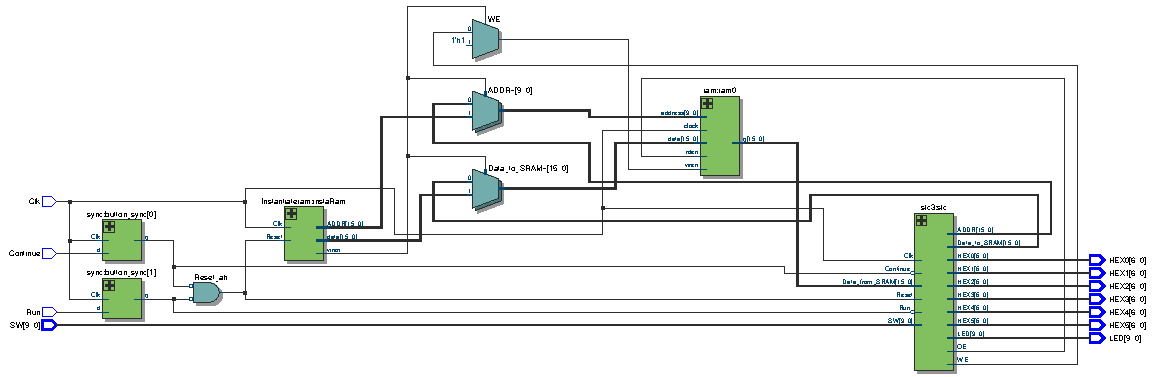
\includegraphics[scale=.9]{toplevel}
        \caption{top level block diagram including MMIO and dedicated SRAM}
    \end{center}
\end{figure}
\begin{figure}[H]
    \begin{center}
1        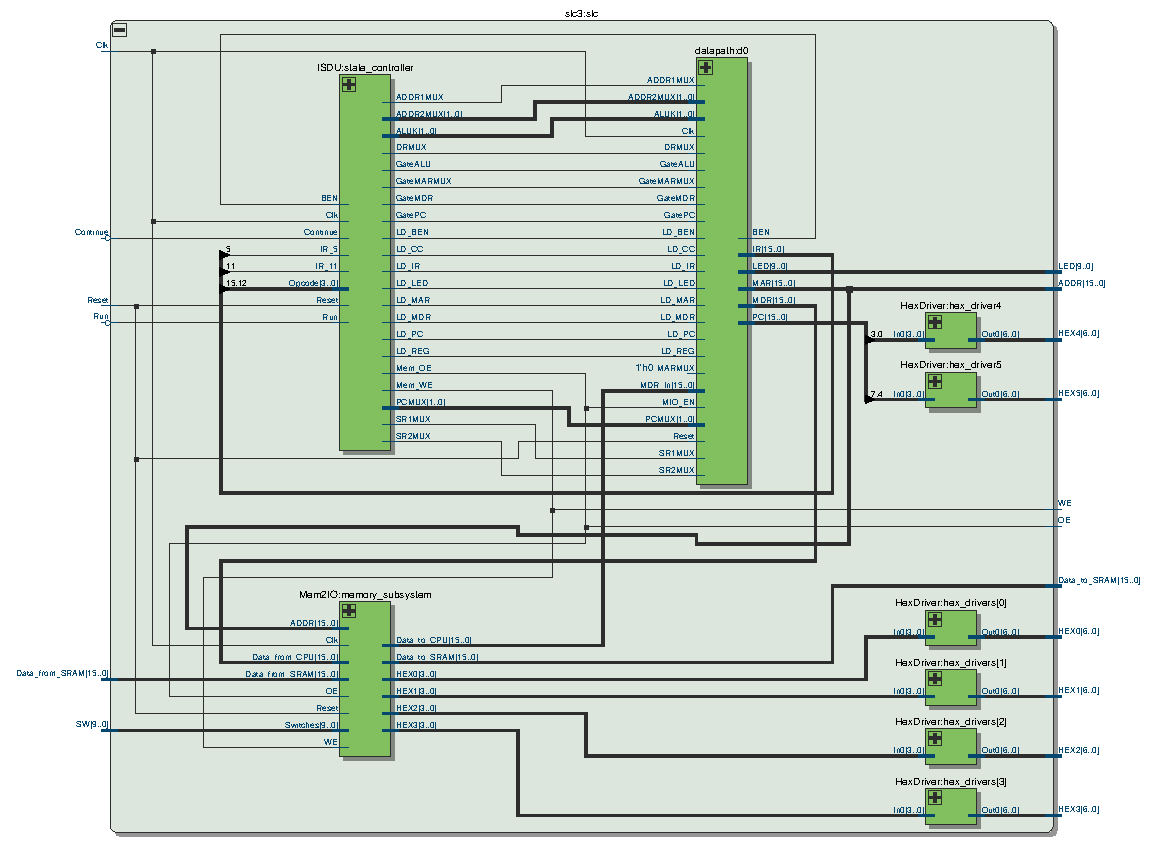
\includegraphics[scale=.9]{slc3}
        \caption{cpu block diagram not including memory and IO}
    \end{center}
\end{figure}
\pagebreak
\label{sec: fsm}
\subsection{State Diagram for Control Unit}
\begin{figure}[h]
    \begin{center}
        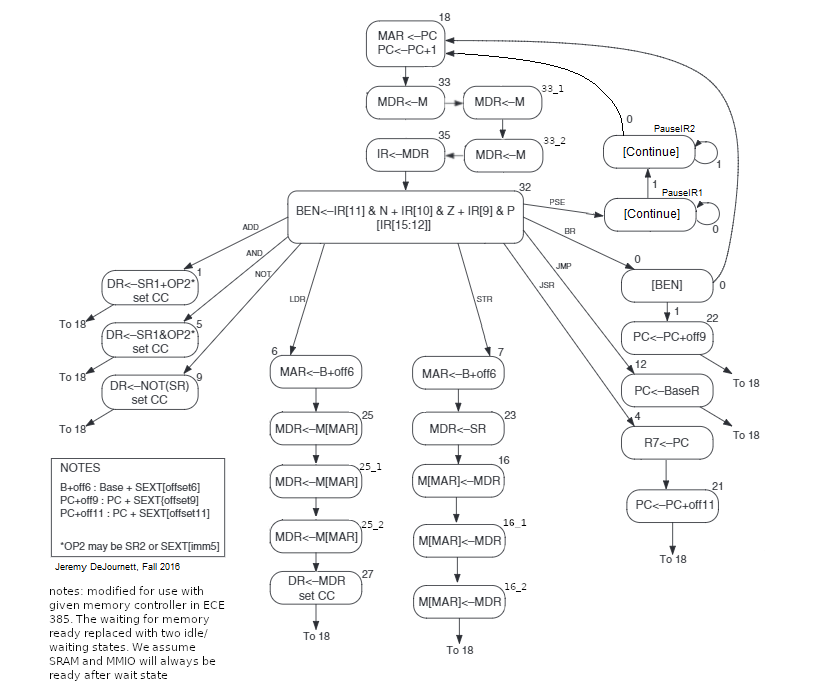
\includegraphics[scale=2.5]{fsm}
        \caption{simplified control unit state diagram. the outputs of each state are not shown and are instead listed below.}
    \end{center}
\end{figure}
\pagebreak
\subsection{CPU control FSM description}
We implement a single cycle control unit using finite state machine. The outputs of the control unit depend on the current state and are listed below: 
%\usepackage{multicol}
\begin{multicols}{2}
\begin{lstlisting}
S_18 :  
	GatePC = 1'b1;
	LD_MAR = 1'b1;
	PCMUX = 2'b00;
	LD_PC = 1'b1;
S_33_1 : //MDR <= M 
	Mem_OE = 1'b1;
S_33_2 : //MDR <= M 
	Mem_OE = 1'b1;
S_33_3 : 
	Mem_OE = 1'b1;
	LD_MDR = 1'b1;
S_35 : 
	GateMDR = 1'b1;
	LD_IR = 1'b1;
PauseIR1:  // LEDs <= ledVect12
	LD_LED = 1'b1; 
PauseIR2: ; // Wait on Continue
S_32 : 
	LD_BEN = 1'b1;
S_01 : //ADD
	SR2MUX = IR_5; // sel imm5
	ALUK = 2'b00; // add
	GateALU = 1'b1;
	LD_REG = 1'b1;
	LD_CC = 1'b1; 
	SR1MUX = 1'b0; //IR[8:6] 
	DRMUX = 1'b1; 
S_00: LD_BEN = 1'b1; 
S_04: 
	GatePC = 1'b1; 
	LD_REG = 1'b1;
	DRMUX = 1'b0; // 111 R7 
S_05:  //AND 
	SR2MUX = IR_5;
	ALUK = 2'b01; //AND
	GateALU = 1'b1;
	LD_REG = 1'b1;
	LD_CC = 1'b1; 
	SR1MUX = 1'b0; //IR[8:6]
	DRMUX = 1'b1; //IR[11:9]
\end{lstlisting}
\columnbreak
\begin{lstlisting}
    //base register B IR[8:6]
S_06, S_07:  //MAR <= B + off6 
	LD_MAR = 1'b1;
	SR1MUX = 1'b0; // IR[8:6]
	ADDR1MUX = 1'b1; //SR1_OUT
	ADDR2MUX = 2'b01; //offset6
	GateMARMUX = 1'b1; 
S_09:  //NOT R(DR) <= ~R(SR1)
	SR2MUX = IR_5; 
	ALUK = 2'b10; //alu_out = ~A
	GateALU = 1'b1; 
	LD_REG = 1'b1;
	LD_CC = 1'b1; 
	SR1MUX = 1'b0; //IR[8:6]
	DRMUX = 1'b1; //IR[11:9]
S_12:  //JMP PC <=BaseR 
	SR1MUX = 1'b0; //IR[8:6]
	LD_PC = 1'b1; 
	PCMUX = 2'b01; //PC_alu_out
	ADDR2MUX = 2'b01; //IR[5:0]
	ADDR1MUX = 1'b1; //reg_SR1
S_16_1, S_16_2, S_16_3: // M[MAR] <= MDR
	Mem_WE = 1'b1;
S_21:  //PC<=PC+off11
	ADDR2MUX = 2'b11; // IR[10:0] off11
	PCMUX = 2'b01; // pc_branch 
	LD_PC = 1'b1; 
S_22:  // PC <= PC + off9 
	ADDR2MUX = 2'b10; // IR[8:0] off9 
	PCMUX = 2'b01; // pc_branch
	LD_PC = 1'b1; 
S_23:  // MDR <= SR 
	ALUK = 2'b11; // A 
	SR1MUX = 1'b1; //IR[11:9]
	GateALU = 1'b1; 
	LD_MDR = 1'b1; 
S_25_1: Mem_OE = 1'b1; // MDR <= M[MAR] 
S_25_2: Mem_OE = 1'b1; // MDR <= M[MAR] 
S_25_3:  // MDR <= M[MAR]
	Mem_OE = 1'b1;
	LD_MDR = 1'b1;
S_27:  // DR <= MDR
	LD_CC = 1'b1; 
	DRMUX = 1'b1; //IR[11:9]
	GateMDR = 1'b1;
	LD_REG = 1'b1;
\end{lstlisting}
\end{multicols}
\pagebreak
\subsection{SystemVerilog Modules}  
% You may insert expanded RTL diagrams of each individual module here if it is legible.
\begin{itemize}
    \item module \verb*|slc3_testtop|
    \subitem this is the top level module for use with testbench simulation. It uses a simulated SRAM module. 
    \item module \verb*|slc3_sramtop| 
    \subitem this is the top level module for use with onboard SRAM on DE10-Lite devboard. It connects the slc3 module to physical SRAM onboard the devboard since it would not be practical to write simulated behavioural SRAM in verilog. 
    \item module \verb*|slc3|
    \subitem implementation of SLC3 ISA, connects the signals from control unit and datapath together to form the basis of the cpu. 
    \item package \verb*|SLC3_2|
    \subitem this systemverilog package contains parameters to convert assembly opcode to machine language opcode. it effectively is a very simple assembler allowing us to directly write assembly like code in our test memory contents. 
    \item module \verb*|register|
    \subitem N bit paramaterized register. supports parallel input, output. loading on rising edge clock. used for registers other than main register file. 
    \item module \verb*|regfile|
    \subitem 8x16 general purpose register file. 3 bits input for DR, SR1, SR2. Used for cpu register file R7:R0
    \item module \verb*|ALU| 
    \subitem Arithmetic logic unit capable of ADD, bitwise AND, bitwise NOT boolean operations. 
    \item module \verb*|mux2_1|
    \subitem paramaterised N bit 2:1 multiplexer used for processor datapath 
    \item module \verb*|mux4_1|
    \subitem paramaterised N bit 4:1 multiplexer used for processor datapath 
    \item module \verb*|mux4_1_onehot|
    \subitem paramaterised N bit 4:1 multiplexer with one hot selection logic. used for data bus. 
    \item module \verb*|Instantiateram|
    \subitem  instantiates on chip SRAM memory for use with Mem2IO MMIO controller. SRAM contents initially contain the test programs to verify the correct functionality of the cpu by testing all the opcode instruction. 
    \item module \verb*|Mem2IO| \label{sec: memcontroller}
    \subitem simple memory controller for cpu, implements MMIO(memory mapped IO) at address 0xffff. Reading or writing to memory address 0x0000 to 0xfffe will read or write to physical onboard SRAM. Writing to MMIO address 0xffff results in the value of the source register specified in the store instruction being written to 7 segment display. Reading from MMIO address 0xffff will read the fpga devboard toggle switch SW[9:0] into the destination register specified in load instruction. The MMIO takes approximiately the same amount of time as SRAM access. In a real CPU the MMIO operation may take much longer than DRAM or SRAM fetch or store, and the control unit of cpu must wait for memory ready signal to continue. Our SLC3 memory controller makes tradeoff of simplicity and fewer logic required at the expense of idle time/speed penalty. 
    \item module \verb*|datapath|
    \subitem  implements LC-3 ISA datapath
    \item module \verb*|ISDU|
    \subitem  implements control finite state machine for LC-3 CPU. see \hyperref[sec: fsm]{CPU control FSM} for the operating principle and description of FSM. 
    \item module \verb*|HexDriver|
    \subitem The hex driver does an encoding by taking in a 4-bit input and outputting a 7-bit active low output corresponding to one hot encoding of the segments on the 7-segment display. 
    \item module \verb*|testbench|
    \subitem testbench is used to generate RTL simulation waveform. It contains sequential instructions to give inputs to top level module in order to jump to individual test programs. see \hyperref[sec: simulation waveform]{simulation waveform} for the exact programs and instructions tested. 
\end{itemize}
\pagebreak
\section{simulation waveform}
\label{sec: simulation waveform}
\begin{figure}[H]
    \begin{center}
        \includegraphics[scale=.35]{test0IO}
        \caption{simulation waveform showing execution of basic IO test program. the 7segment display displays the hexadecimal value of the toggle switch input. You can see the 7segment one hot active low output for each of the digits represent the switch input as well as the switch value loaded into R1 through MMIO.}   
    \end{center}
\end{figure}
\begin{figure}[H]
    \begin{center}
        \includegraphics[scale=.28]{test1IO}
        \caption{simulation waveform showing execution of basic IO test program with pause state. the 7segment display is updated with hexadecimal value of toggle switch input every time continue is pulled low during pauseIR state. You can see the 7segment one hot active low output for each of the digits represent the switch input as well as the switch value loaded into R1 through MMIO.}   
    \end{center}
\end{figure}
\begin{figure}[H]
    \begin{center}
        \includegraphics[scale=.3]{testloadstore}
        \caption{simulation waveform showing self modifying code load store test program. the LED register output is increase every time continue is pulled low during pauseIR state.}   
    \end{center}
\end{figure}
\begin{figure}[H]
    \begin{center}
        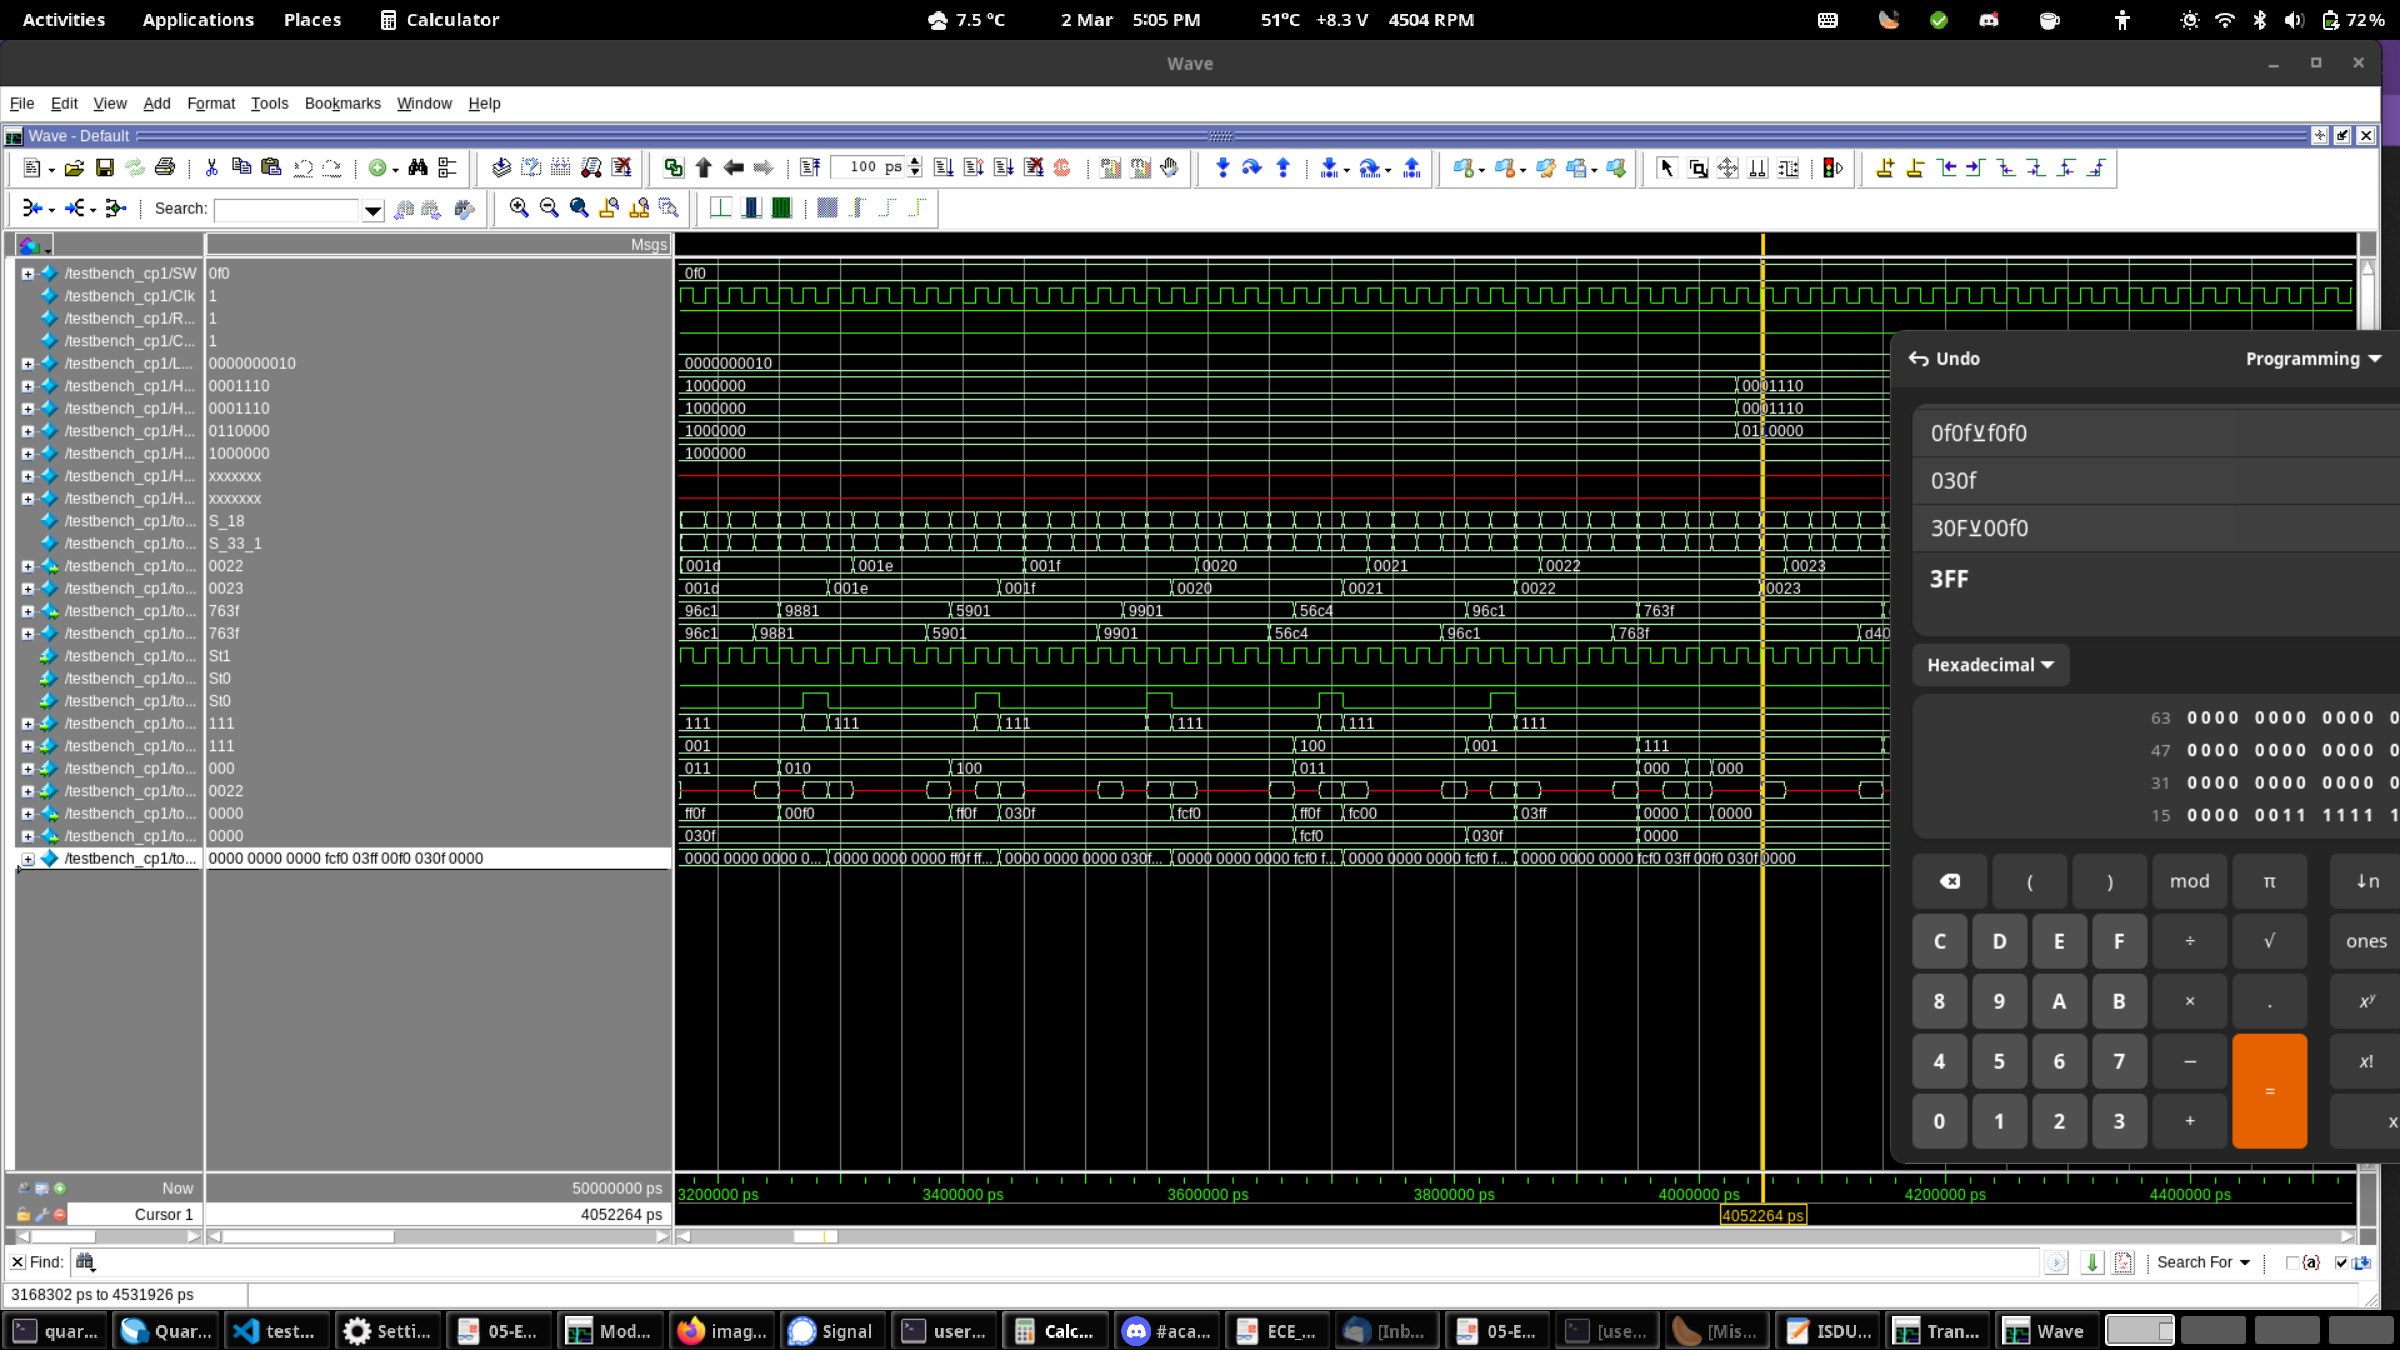
\includegraphics[scale=.3]{xor_asm}
        \caption{simulation waveform showing the bitwise xor calculation using the AND, NOT operation of ALU. the inputs A = 0x030f and B = 0x00f0 are stored in R1, R2, and output 0x03ff is stored in R3 before output to 7segment display using MMIO store operation}   
    \end{center}
\end{figure}
\begin{figure}[H]
    \begin{center}
        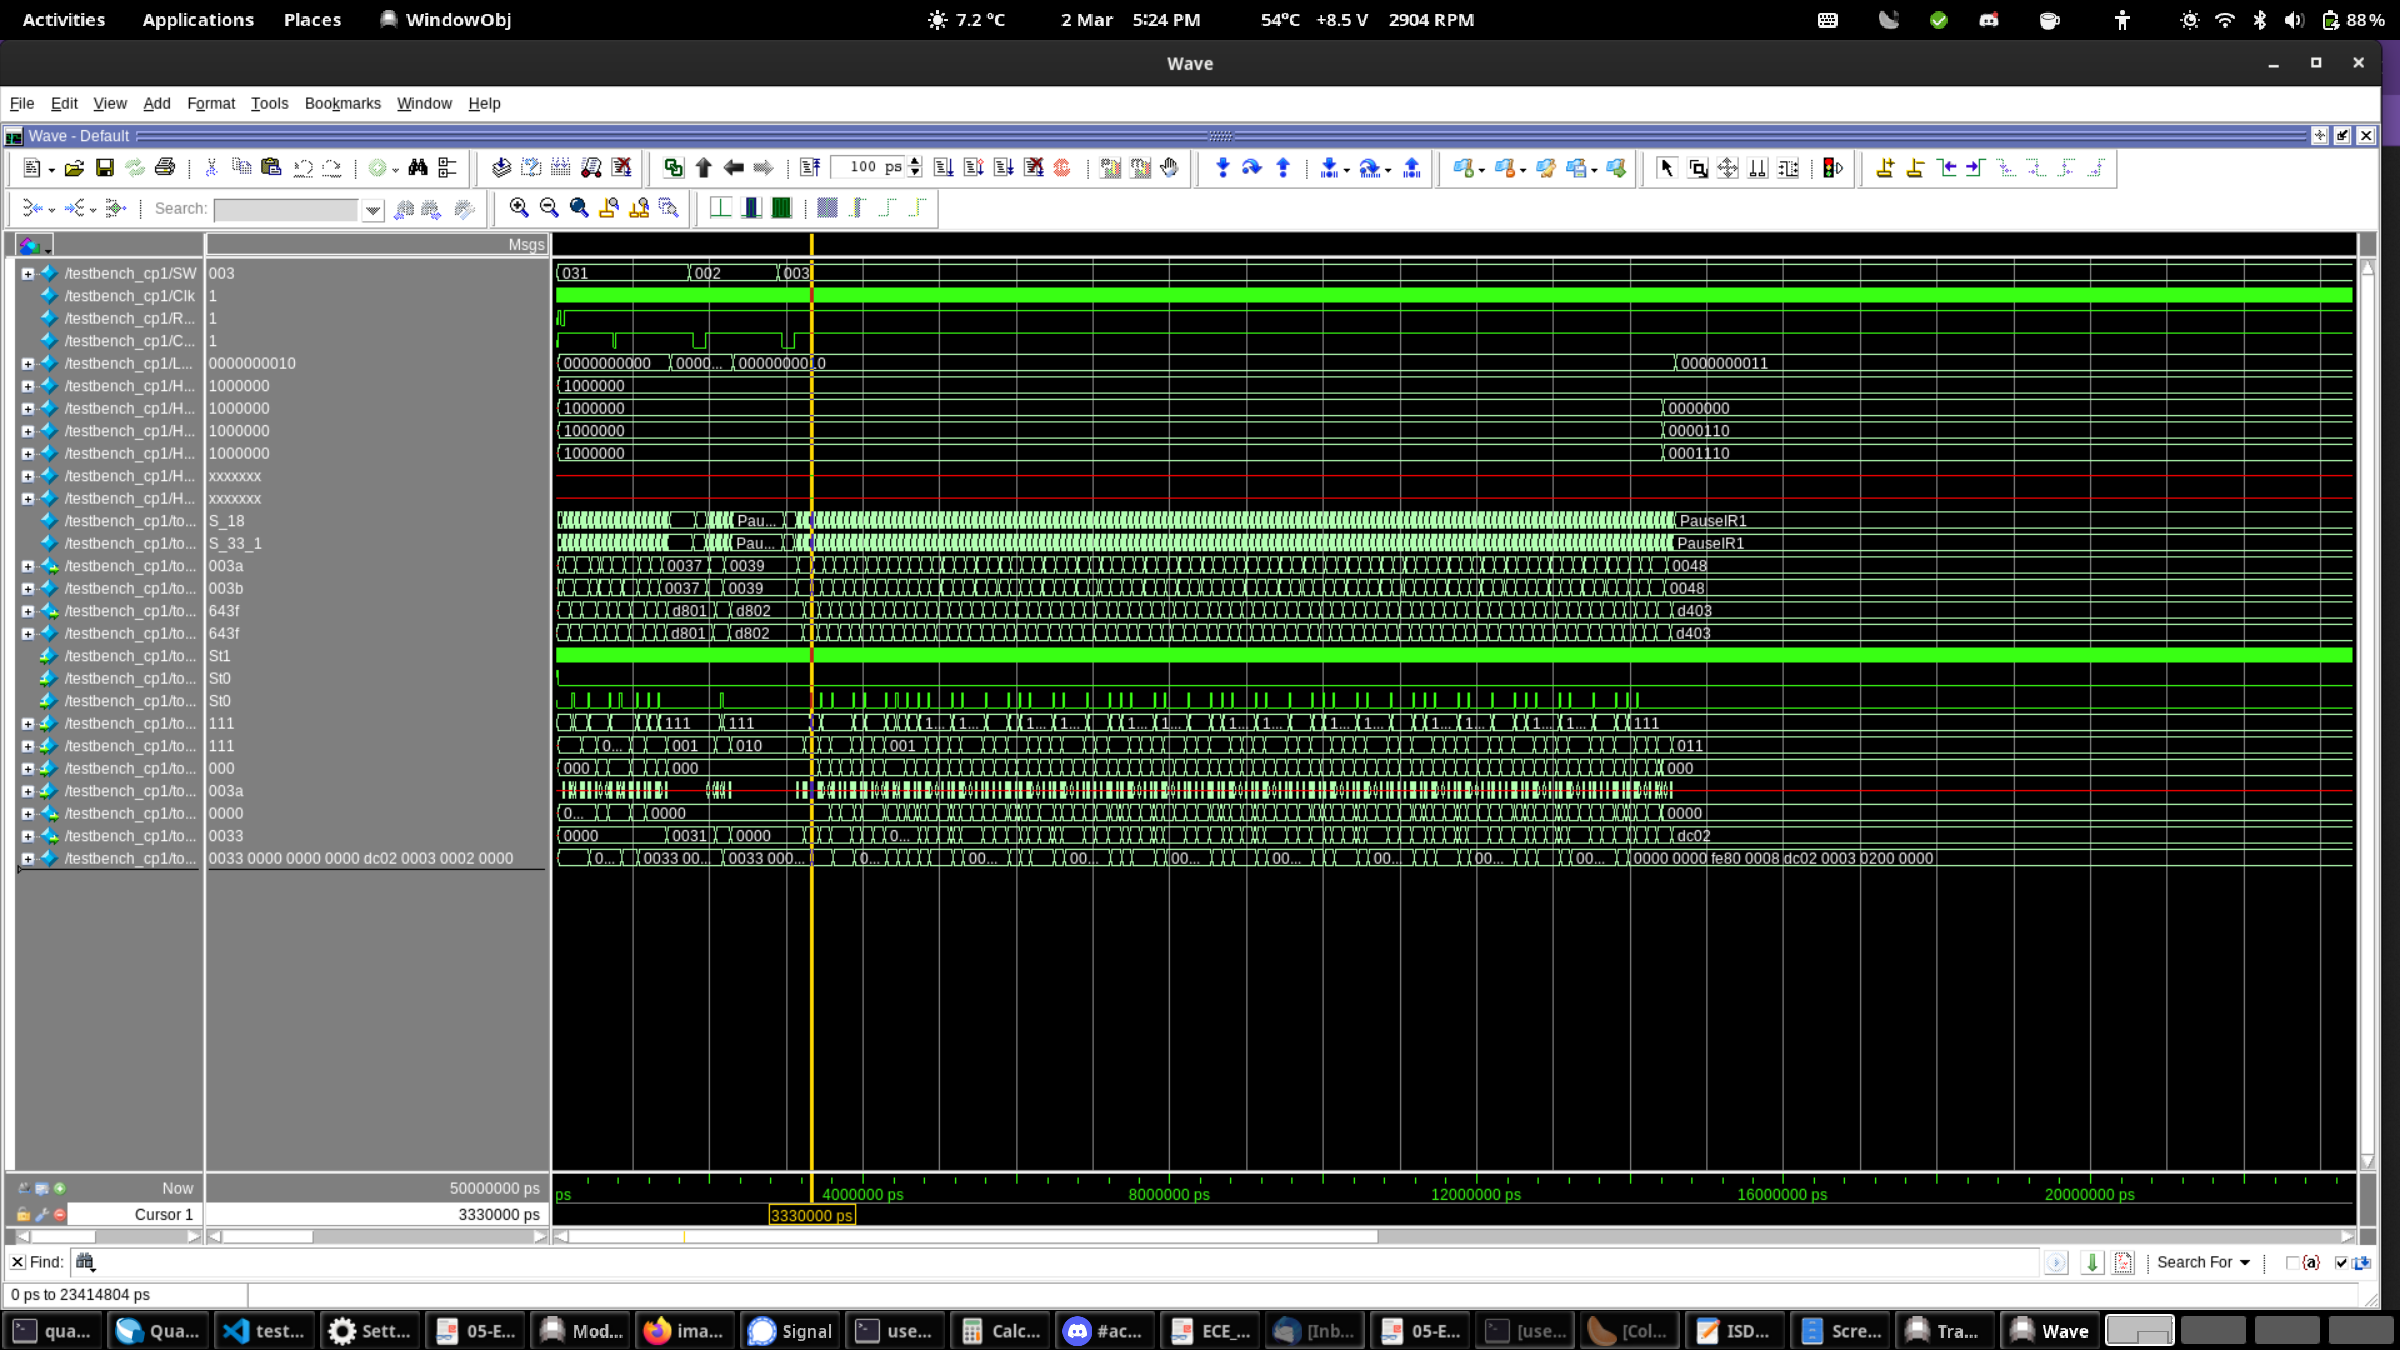
\includegraphics[scale=.3]{mul_asm}
        \caption{simulation waveform showing mulitiplication operation performed using add shift algorithm. the inputs A = 0x0002 and B = 0x0003 are stored in R1, R2, and output is stored in R3 before output 0x0008 to 7segment display using MMIO store operation}   
    \end{center}
\end{figure}
\begin{figure}[H]
    \begin{center}
        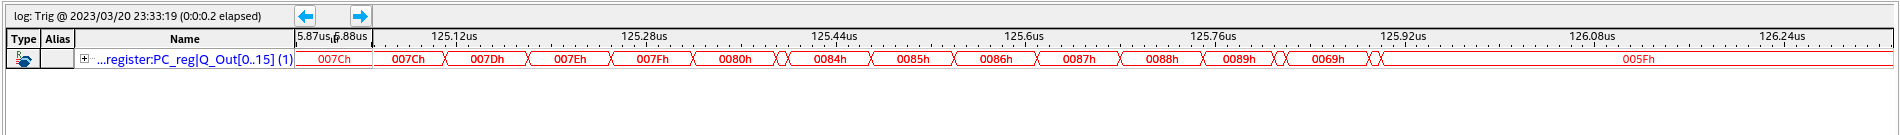
\includegraphics[scale=.3]{sort_computation1}
        \caption{simulation waveform showing the execution of sorting program. The given data is used }   
    \end{center}
\end{figure}
The use of RTL simulation allows us to view intermediate data signal in between module as well as the final output of the top level processor module. This is useful when troubleshooting incorrect final output. For example, we were able to see that our active low reset was always holding our register unit in reset due to incorrect inversion logic, and see the values of every single register at once. By starting with testing individual instruction and building up to full programs it is possible to isolate incorrect logical implementation of datapath or control signal. 
\pagebreak
\section{Post Lab}
%What is MEM2IO used for, i.e. what is its main function? 
MEM2IO is the memory controller that implements MMIO and SRAM read write functionality. See \hyperref[sec: memcontroller]{Mem2IO module decription} for details regarding its operation, implementation, and design tradeoff between speed and simplicity. 
\newline

%difference between br jmp
Both the branch (\verb*|BR|), jump (\verb*|JMP|), and jump subroutine (\verb*|JSR|) functions will modify the instruction pointer register (PC), but they are used for different purpose. \newline 
The JMP instruction unconditionally jumps to address specified in source register. It is used when unconditionally jump to a address that cannot be expressed as PC+imm9. This can be needed when executing a program from an operating system or shell. \newline 
The JSR instruction unconditionally jumps to PC+imm11 and stores the current instruction pointer into R7. This is used when calling subroutine where you must preserve the base instruction pointer in R7 to return after completion of subroutine.\newline
Finally the BR instruction conditionally branches to PC+imm9 based on the condition codes specified in IR[11:9]. This is used for evaluating if statements, loops and similar constructs in high level programming language. \newline

%What is the purpose of the R signal in Patt and Patel? How do we compensate for the lack of the signal in our design? What implications does this have for synchronization?
The R signal in the Patt and Patel book LC3 specification is the memory ready signal from the memory controller. As discussed in \hyperref[sec: memcontroller]{Mem2IO module decription} our memory controller does not implement ready signal to reduce complexity. We compensate for the lack of memory ready signal in our control FSM by introducing multiple wait/idle state in every memory operation. We discovered that we need up to four states to account for stable operation in all power/signal integrity condition. This workaround is stable but wastes time where the cpu is idle for longer than necessary when waiting on memory to become ready. A more robust approach would be for the memory controller to output a ready signal when the memory or MMIO data is ready, and the fsm to immediately proceed to the next state when such signal is asserted. This will maintain perfect synchronisation between processor and memory which will be more fast and stable. In addition, if slower MMIO devices are later added, it will be necessary to assert ready signal since the access latency for MMIO and SRAM may be orders of magnitude apart. \newline
\subsection{performance statistics}
\begin{tabular}{ l l }
LUT & 1366\\  
DSP & 0\\  
BRAM Memory (bits) & 27648\\
Flip-Flop & 823\\  
Frequency(MHz) & 108.48\\ 
Static Power(mW) & 89.95\\  
Dynamic Power(mW) & 1.33\\  
Total Power(mW)) & 100.20 
\end{tabular} 
\subsection{instructions per second calculations}
In order to benchmark the performance of our processor design in millions of instructions per second or MIPS(not to be confused with the MIPS ISA) we use the SignalTap integrated logic analyser to capture waveform of the instruction pointer (PC) register during known programs. We can then count the number of instructions executed over a known time frame and use the average of multiple runs and multiple different programs to approsimate the MIPS achieved by our design. We cannot use simulator for calculating real world performance because simulation is not able to accurately predict real world performance like a logic analyser and real hardwawre(FPGA) can. We discuss ways we can improve the performance of our design in the conclusion. 
\subsubsection{xor program MIPS}
The XOR test program computation instructions (not including the MMIO input instructions) is stored in test memory addresses 0x001a to 0x0029. We can simply subtract the two instruction pointers to see that there are 15 computation instructions because there is no branch or jump instruction in this computation. \newline
The computation takes 650 ns to run therefore the xor computation runs at 23.07 MIPS.
\begin{figure}[H]
    \begin{center}
        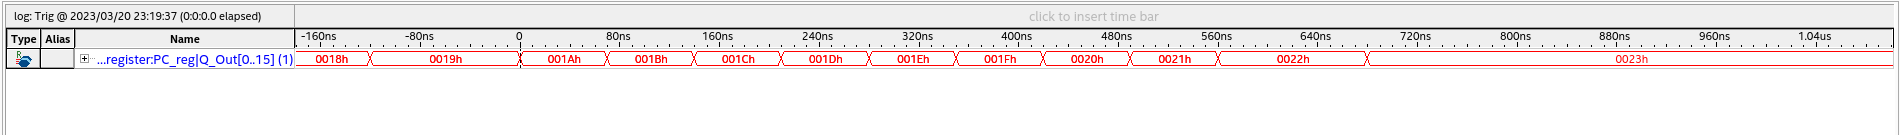
\includegraphics[scale=.3]{xor_computation}
        \caption{SignalTap waveform of xor computation running on actual hardware FGPA}   
    \end{center}
\end{figure}
\subsubsection{multiplication program MIPS}
The multiplication test program computation instructions is stored in test memory addresses 0x003a to 0x0047. Including the add-shift loop branch condition there are 104 instructions. The add shift loop runs 8 times regardless of inputs so the number of instructions is constant regardless of input to the program. \newline
The computation takes 5.9 $\mu$s to run therefore the multiplication computation runs at 17.63 MIPS.
\begin{figure}[H]
    \begin{center}
        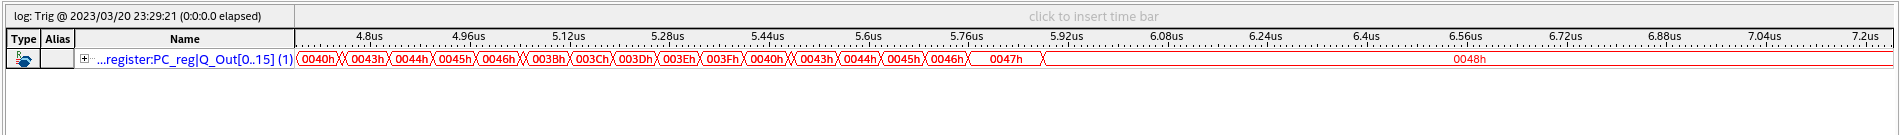
\includegraphics[scale=.3]{mul_computation0}
        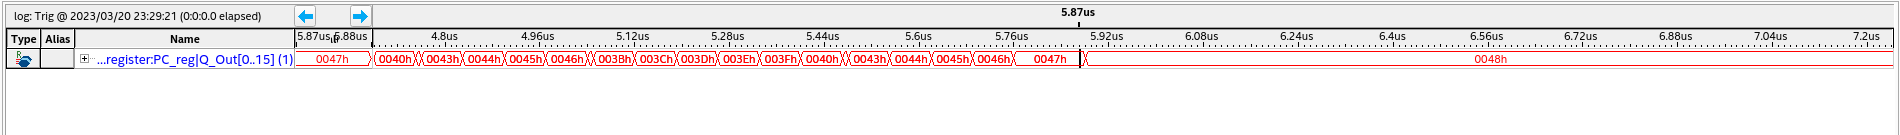
\includegraphics[scale=.3]{mul_computation1}
        \caption{SignalTap waveform of multiplication computation running on actual hardware FPGA }   
    \end{center}
\end{figure}
\subsubsection{sorting program MIPS}
The sorting test program computation instructions is stored in test memory addresses 0x0077 to 0x0089. There are two nested loops both with index i = 16. We can conclude that the computation of sorting program takes 0x10*0x10*(0x89-0x77) = 0x1200 = $4608_{10}$ \newline
The computation takes 126 $\mu$s  to run therefore the sorting computation runs at 36.57MIPS.
\begin{figure}[H]
    \begin{center}
        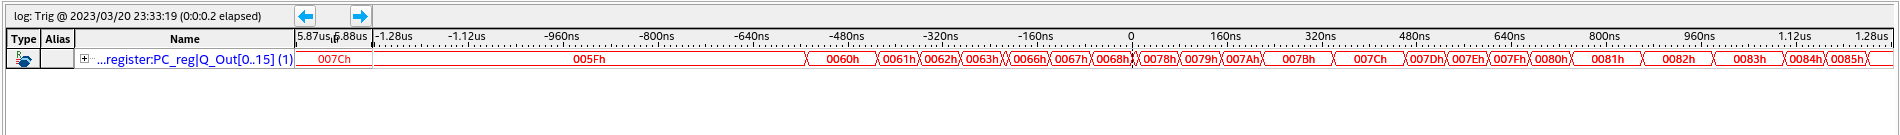
\includegraphics[scale=.3]{sort_computation0}
        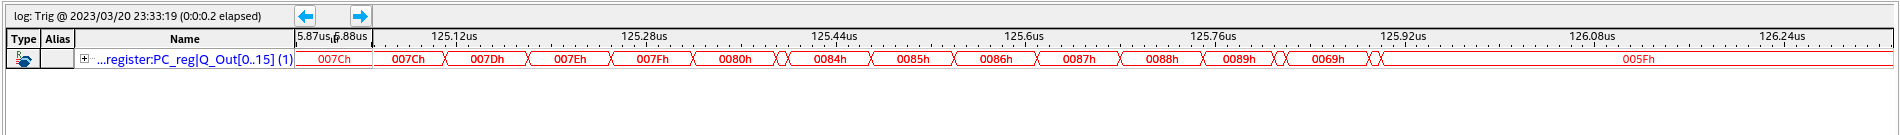
\includegraphics[scale=.3]{sort_computation1}
        \caption{SignalTap waveform of sorting computation running on actual hardware FPGA}   
    \end{center}
\end{figure}

From the 3 samples collected we can approximate the average performance of our design to be 25.76 MIPS.
\section{Conclusion}
We were able to achieve a fully functional LC3 microprocessor with all instructions behaving as expected. If we had more time, we would have done some further optimisations to our design to increase performance and stability. For example, we can  modify our memory controller to assert a ready signal when the memory or MMIO operation is complete. This will reduce the number of FSM states significantly since we avoid many arbitary idle waiting states associated with each memory operation, i turn decreasing gate count because we need fewer states to enumerate in the FSM as well simplified next state logic. Another more complicated optimisation of our design can be to use pipelining to speed up the processor with parallel computing.\newline
The lab documentation was reasonably easy to understand for anyone with some background in computer architecture. Some of the multiplexer input might have been slightly unclear which input correspond to which selection, but as long as it is consistent between datapath and control unit the order does not really matter. The memory controller operation was also slightly unclear because we were instructed to use a workaround for lack of memory ready signal, and it was not clear exactly how long the control FSM should wait for memory controller IO to become ready. 
\end{document}